\newpage
\section{Lightmapped texture baking}
\label{sec:chapter_lrl_li_te_ba}

Nel paragrafo \ref{sec:chapter_stato_arte_lightmap} si è già discusso di lightmap, e di come queste vengono realizzate.
Le lightmapped texture sono di base delle lightmap, ma con delle differenze sia nelle proprietà che nel processo costruttivo. 
\\
Come già accennato nell’introduzione, per il baking di queste lightmapped texture si è fatto uso di uno strumento esterno in grado di computare algoritmi di illuminazione complessi senza coinvolgere il real-time rendering di Three JS. La scelta è ricaduta sul software di grafica 3D Blender, il quale dispone di algoritmi di illuminazione indiretta per una resa grafica notevole, come il Path Tracing. Inoltre la realtà open source del programma ha permesso di modellarne dei comportamenti, per venire incontro a delle esigenze di utilizzo che verrano mostrate nei capitoli più avanti. Blender permette di eseguire l’unwrap dei modelli 3D e quindi di produrre le mappe UV di cui si è già discusso nel paragrafo \ref{sec:chapter_stato_arte_lightmap}. 
\\
\begin{figure}[htb]
 \centering
 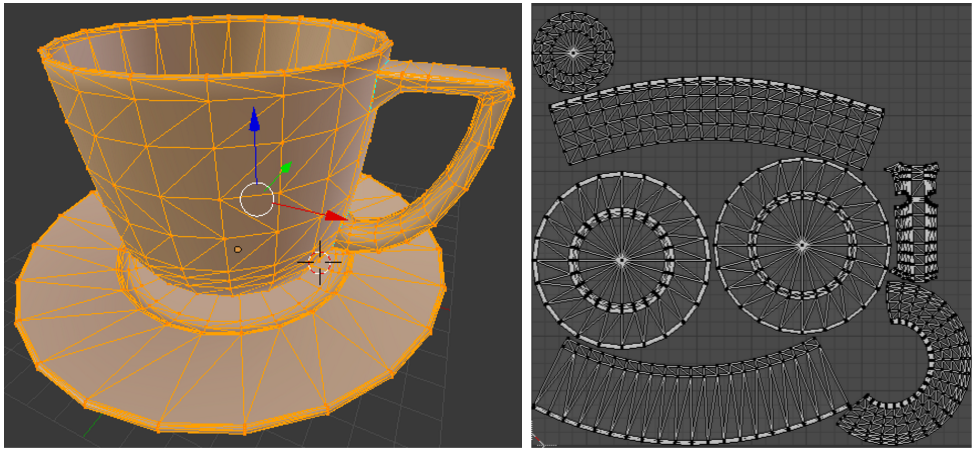
\includegraphics[width=1\linewidth]{images/chapter_lrl/lrl_unwrap.png}\hfill
 \caption[Blender unwrap]{Processo di unwrap in Blender.}
 \label{fig:lrl_unwrap}
\end{figure}
Il processo di baking delle lightmap prevede nella stragrande maggioranza dei casi che le UV Map utilizzate siano quelle generate dal software in uso. Ci sono tuttavia dei casi dove questa potrebbe non essere la soluzione ottimale.
Quando si crea una scena è possibile importare dei modelli creati da terze parti; ogni modello è rappresentato da un file obj contenente le primitive geometriche del modello (vertici, spigoli e facce), le coordinate UV, e le normali. Inoltre al file obj viene allegata la diffuse texture pensata per il modello dal creatore dello stesso.
Le coordinate UV del modello sono realizzate per consentire un mapping ottimale della diffuse texture sulle superfici 3D dell’oggetto. Siccome quindi l’UV Map già esiste, ed è ottimizzata per il modello, è possibile esulare Blender dall’eseguire l’unwrap, evitando quindi di generare una mappa UV diversa, a favore di quella preesistente. 
Ovviamente qualora mancasse la mappa UV di un modello, l’unwrap sarà necessario. 
Utilizzando per la lightmap la stessa UV Map usata per mappare la diffuse texture si avrà che:  se un texel $T$ nella diffuse texture copre la posizione $(u1,v1)$, e un lumel $L$ copre la stessa posizione $(u1,v1)$ nella lightmap, allora $L$ e $T$ saranno mappati sullo stesso frammento del modello 3D.
Quindi diffuse texture e lightmap sono completamente sovrapponibili, e il mapping sul modello 3D sarà ottimale per le lightmap così come lo è per la diffuse texture.
I vantaggi di una scelta simile sono soprattutto a livello qualitativo. 
Nel paragrafo \ref{sec:chapter_stato_arte_lightmap} si è già fatto cenno a come i software di grafica 3D permettano all’artista di intervenire sul processo di unwrap, per modellare a mano l’UV map generata dal software nei punti dove il mapping può aver commesso degli errori; questo può accadere con geometrie complesse, specialmente in punti dove la superficie del modello è curva. 
Nel presente lavoro di tesi si assume che la mappa UV realizzata dal creatore del modello sia quella ottimale, in quanto creata appositamente per quell’oggetto. Una procedura completamente automatizzata infatti difficilmente riuscirebbe a raggiungere lo stesso risultato.
\\
\begin{figure}[htb]
 \centering
 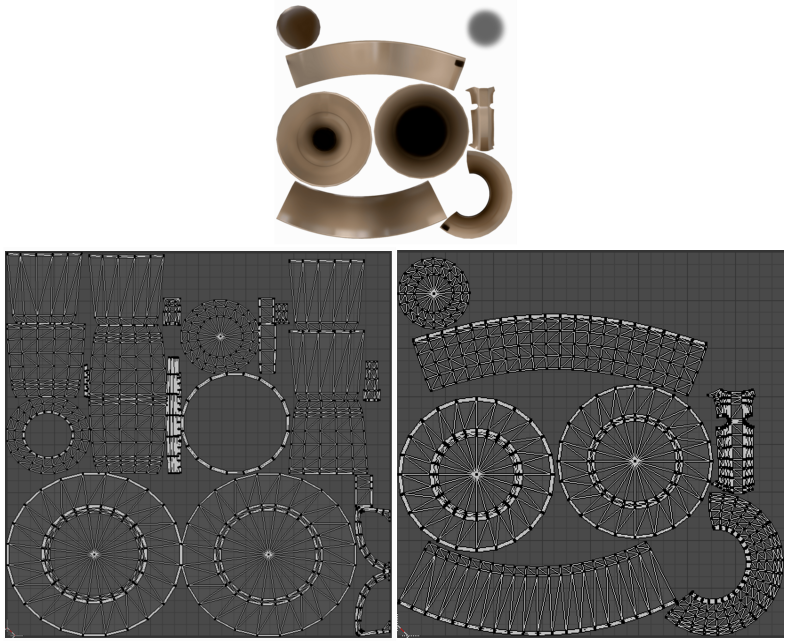
\includegraphics[width=1\linewidth]{images/chapter_lrl/lrl_diff_uvmap.png}\hfill
 \caption[Confronto UV Map]{In foto viene mostrata una mappa uv generata automaticamente da Blender (a sinistra), e una mappa uv creata dall'artista del modello (a destra).}
 \label{fig:lrl_diff_uvmap}
\end{figure}
Nel contesto del presente elaborato di tesi il software di grafica 3D è completamente trasparente all’utente. Pertanto le uniche UV Map in possesso sono quelle generate da Blender in modo completamente automatico o quelle create da terzi per i modelli importati, per le quali invece il creatore potrebbe aver avuto la possibilità di intervenire a mano per migliorarle.
\\
Generalmente le informazioni luminose calcolate offline vengono memorizzate in una struttura dati separata dalla diffuse texture, in modo da poter usare l’una indipendentemente dall’altra, e sfruttare la riusabilità delle diffuse texture.
\\ 
Tuttavia allo stato attuale è previsto un unico setup di illuminazione all’interno della scena, anche se la flessibilità del sistema permetterebbe l’installazione di un supporto per diversi setup di illuminazione all’interno della stessa scena, come il ciclo giorno/notte.  Avere per uno stesso appartamento setup di illuminazione diversi è utile specialmente per branche dell’architettura come l’illuminotecnica. Pertanto il fattore riusabilità di una texture, di cui si è fatto cenno nel paragrafo \ref{sec:chapter_stato_arte_lightmap}, diventa superfluo. 
\\
\begin{figure}[htb]
 \centering
 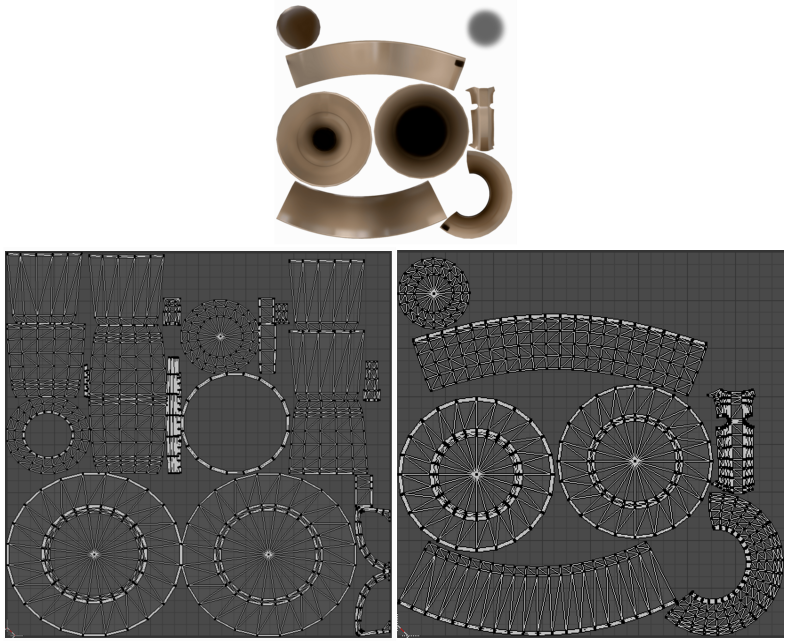
\includegraphics[width=1\linewidth]{images/chapter_lrl/lrl_diff_uvmap.png}\hfill
 \caption[Confronto UV Map]{In foto viene mostrata una mappa uv generata automaticamente da Blender (a sinistra), e una mappa uv creata dall'artista del modello (a destra).}
 \label{fig:lrl_diff_uvmap}
\end{figure}
\\
In questo caso ha poco senso mantenere elementi di immagine e di luce in strutture dati separate, e quindi grazie alla sovrapponibilità delle due strutture dati si può ottenere un’unica texture dove in ogni texel i valori RGB della diffuse texture sono moltiplicati per i valori di irradianza memorizzati nei lumel della lightmap. Questa nuova struttura dati viene detta lightmapped texture. 
\\
\begin{figure}[htb]
 \centering
 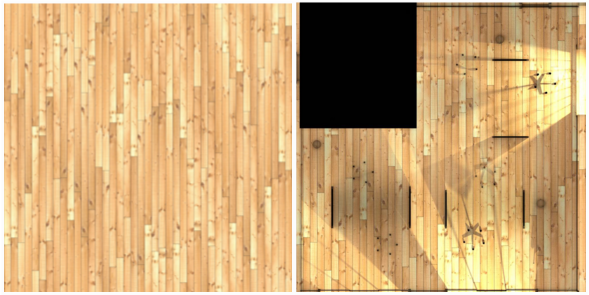
\includegraphics[width=1\linewidth]{images/chapter_lrl/lrl_li_te.png}\hfill
 \caption[Lightmapped texture]{Confronto tra una normale diffuse texture (a sinistra), e relativa lightmapped texture (a destra)}
 \label{fig:lrl_li_te}
\end{figure}
Il software Blender permette la creazione di lightmapped textures, specificando la modalità di bake “combined”; questa modalità emula ciò che si avrebbe con render completo del modello, e quindi produce in output la combinazione tra luce e colore diffuse del modello.